% Use either your LaTeX editor or latexmk to compile.

\documentclass[a4paper, 12pt]{article}

% Document quality things
\usepackage[utf8]{inputenc}
\usepackage{microtype, xcolor}
\usepackage{url, hyperref}
\hypersetup{colorlinks=true, linkcolor=blue, citecolor=black, urlcolor=blue}

% Image-related packages
\usepackage{graphicx}
\usepackage{float}
\graphicspath{ {./detailed-design-diagrams/} }
\usepackage[font=small,skip=5pt]{caption}

% Setting margins
\usepackage[a4paper, left=2cm, right=2cm, top=1.75cm, bottom=1.75cm, includefoot]{geometry}

% Table helper packages
\usepackage{multirow, multicol}
\usepackage{makecell}
\usepackage{array}
%\usepackage{tabularx} % Not needed currently, but has a few nice options
%\usepackage{wrapfig} % Floating figures/tables

% Prevents spamming tedious newlines everywhere, also disables auto indentation, etc.
\usepackage[skip=0.75\baselineskip plus 2pt]{parskip}

% Self-explanatory
\usepackage{titlesec}
\titleformat{\section}[block]{\normalfont\scshape\Large}{\thesection}{1em}{}
\titleformat{\subsection}{\normalfont\large}{\thesubsection}{1em}{}

% Referencing
\usepackage[backend=bibtex, style=numeric-comp, sorting=none]{biblatex}
\addbibresource{bibliography.bib}

\begin{document}
    
    % Header Table
    \begin{table}[h!]
        \renewcommand{\arraystretch}{3}
        \centering
        \begin{tabular}{ | >{\raggedleft\arraybackslash}m{3cm} l >{\raggedleft\arraybackslash}m{3cm} m{3cm} | }
            \hline
            \Huge CS 102 & \textit{Spring 2020/21} & \multirow{2}{*}{\makecell{Project\\Group}} & \multirow{2}{*}{\textbf{\Huge G2C}} \\
            \makecell[r]{Instructor:\\Assistant:} & \makecell[l]{\textbf{Aynur Dayanık}\\\textbf{Haya Shamim Khan Khattak}} & & \\
            \hline
        \end{tabular}
    \end{table}
    
    % Grading Table
    \begin{table}[h!]
            \renewcommand{\arraystretch}{1.4}
            \centering
            \footnotesize
            \begin{tabular}{ l p{1.5cm} | p{1.5cm} | }
                \hline
                \multicolumn{1}{|c|}{\textbf{Criteria}} & \multicolumn{1}{c|}{\textbf{TA/Grader}} & \multicolumn{1}{c|}{\textbf{Instructor}} \\ \hline
                \multicolumn{1}{|p{10.5cm}|}{Presentation} &  &  \\[10ex] \hline
                \multicolumn{1}{r|}{\textbf{Overall}} &  &  \\
                \cline{2-3}
            \end{tabular}
    \end{table}
    
    % Project Information Header
    {\centering\Huge \bfseries \raisebox{0.5ex}{\texttildelow} LabConnect \raisebox{0.5ex}{\texttildelow} \par}
    
    \begin{table}[h!]
        \renewcommand{\arraystretch}{1.4}
        \centering
        \small
        \begin{tabular}{ r l }
            \textbf{Borga Haktan Bilen} & 22002733 \\
            \textbf{Vedat Eren Arıcan} & 22002643 \\
            \textbf{Berkan Şahin} & 22003211 \\
            \textbf{Berk Çakar} & 22003021 \\
            \textbf{Alp Ertan} & 22003912 \\
        \end{tabular}
    \end{table}
    
    % Document Type Header Table
    \begin{table}[h!]
        \renewcommand{\arraystretch}{1.5}
        \centering
        \begin{tabular}{ |>{\centering\arraybackslash}m{15.15cm}| }
            \hline
            \Large \textbf{Detailed Design Report} \\
            \small (version 2.0) \\
            \small \textbf{\today} \\
            \hline
        \end{tabular}
    \end{table}
    
    % Document begins here...
    
    \section{Introduction}
    
    LabConnect facilitates communication between students, TA's, tutors,
    and instructors. In the background, it is a web application
    that aims to assist CS introductory courses in organization and communication. 
    Proposed ideas for features include priority queuing for TA zoom rooms among many other 
    enhancements to TA/instructor productivity. For example, those who have completed their labs 
    can be tested using pre-defined (by TA or instructor) unit tests,  
    and then placed into a queue to optimize the TA-student meeting arrangement process in general. 
    Much of the repetitive work that course staff need to do can be reduced substantially by automated actions,
    allowing TA's and tutors to allocate more time for more hands-on help towards students.
    In summary, LabConnect is a developing project that aims to make education more productive for students,
    and more efficient for teaching staff, above all.
    
    \section{System Overview}
    
    \subsection{Organisation \& Architecture}
    
    Shown below is the diagram of the organization of LabConnect's architecture.
    Users of varying roles interact with the interface displayed using the ReactJS library, which also makes
    HTTP requests to the REST API powered by the Spring framework, over the internet.
    The Spring framework acts mostly as the controller segment of the project, delivering data
    that is obtained through model classes and their communication with the databases.
    
    \begin{figure}[H]
        \centering
        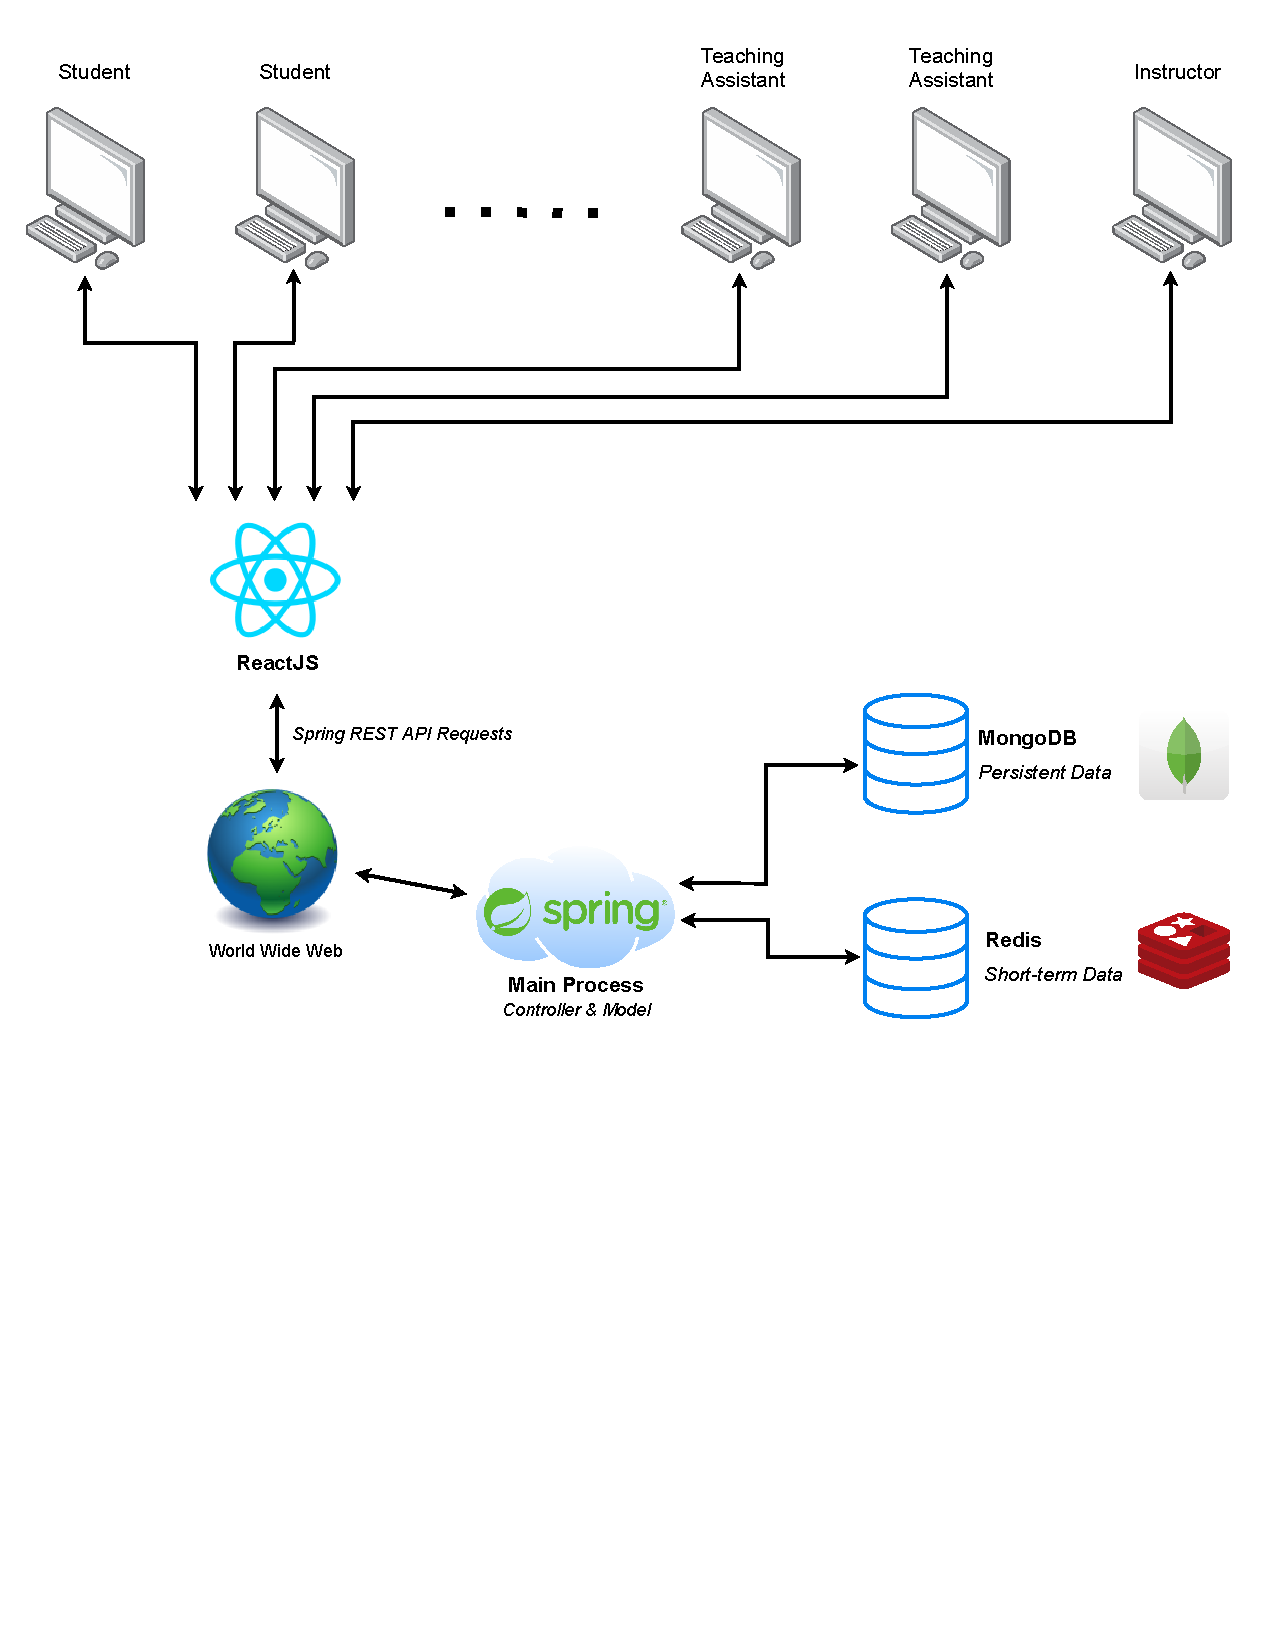
\includegraphics[width=\textwidth]{organization}
        \caption{Overview of LabConnect's Organisation}~\label{fig:organisation-diagram}
    \end{figure}
    
    \pagebreak
    
    \subsection{Technologies}
    
    \subsubsection{Back-end}
    
    \begin{itemize}
        \item \textbf{Spring} - Framework to be used to power the REST API at the /api/ data endpoint.
              All necessary data will be exposed at the API endpoint, but only with proper authentication.
              Requests are only authorized accordingly with the user's account permission level.
              The \textit{Spring Security} and \textit{Spring MVC} frameworks may also be taken advantage of.
        \item \textbf{MongoDB} - To be used as persistent storage; account data, assignment data, etc.
        \item \textbf{Redis} - To be used as short-term storage; user session, authentication, etc.
    \end{itemize}
    
    \subsubsection{Front-end}
    
    \begin{itemize}
        \item \textbf{SASS} - Useful preprocessor to write CSS more productively.
        \item \textbf{ReactJS} - Will be used to construct a single-page-app user interface,
              which will serve components according to the API call responses.
    \end{itemize}
    
    \subsubsection{Build \& Utility Tools}
    
    \begin{itemize}
        \item \textbf{Spring Boot} - May be used to simplify the development of Spring components.
        \item \textbf{Maven} - Build automation tool, good for any medium to large scale project.
        \item \textbf{Docker} - Facilitates the deployment of the project, and it may
              also be viable to use \textit{docker-compose} to deploy separate containers
              for databases and other components simultaneously.
    \end{itemize}
    
    \subsubsection{Domain \& Host}
    
    \begin{itemize}
        \item \textbf{Domain} - \textit{labconnect.me} is the proposed domain for the website.
        \item \textbf{Hosting} - The project will most likely be run on either a container deployment service,
              or a VPS service.
    \end{itemize}
    
    \pagebreak

    \section{Core Design Details}
    
    Most of the data, being of persistent nature, is stored in a database. But the model classes
    perform the necessary queries and subsequent actions to the data as necessary,
    essentially grouping database queries logically. Additionally, model classes are also responsible for serving
    functionallity (service layer) to the controller layer which then controller layer handles HTTP requests (GET, POST, DELETE, PUT) in order 
    to create a REST API. In the class diagram below [\ref{fig:class-diagram}], all the Java classes, 
    interfaces and enums are showed with their relations. However, because of the magnitude of the project 
    the diagram below might not be clear enough to examine. Thus, we uploaded the UML diagram 
    (with magnification script) and Javadocs to the LabConnect website under a new distinct subdomain for convience. 
    Links for these are respectively: \href{http://docs.labconnect.me/uml/}{http://docs.labconnect.me/uml/} 
    and \href{http://docs.labconnect.me/}{http://docs.labconnect.me/}.

    \begin{figure}[H]
        \centering
        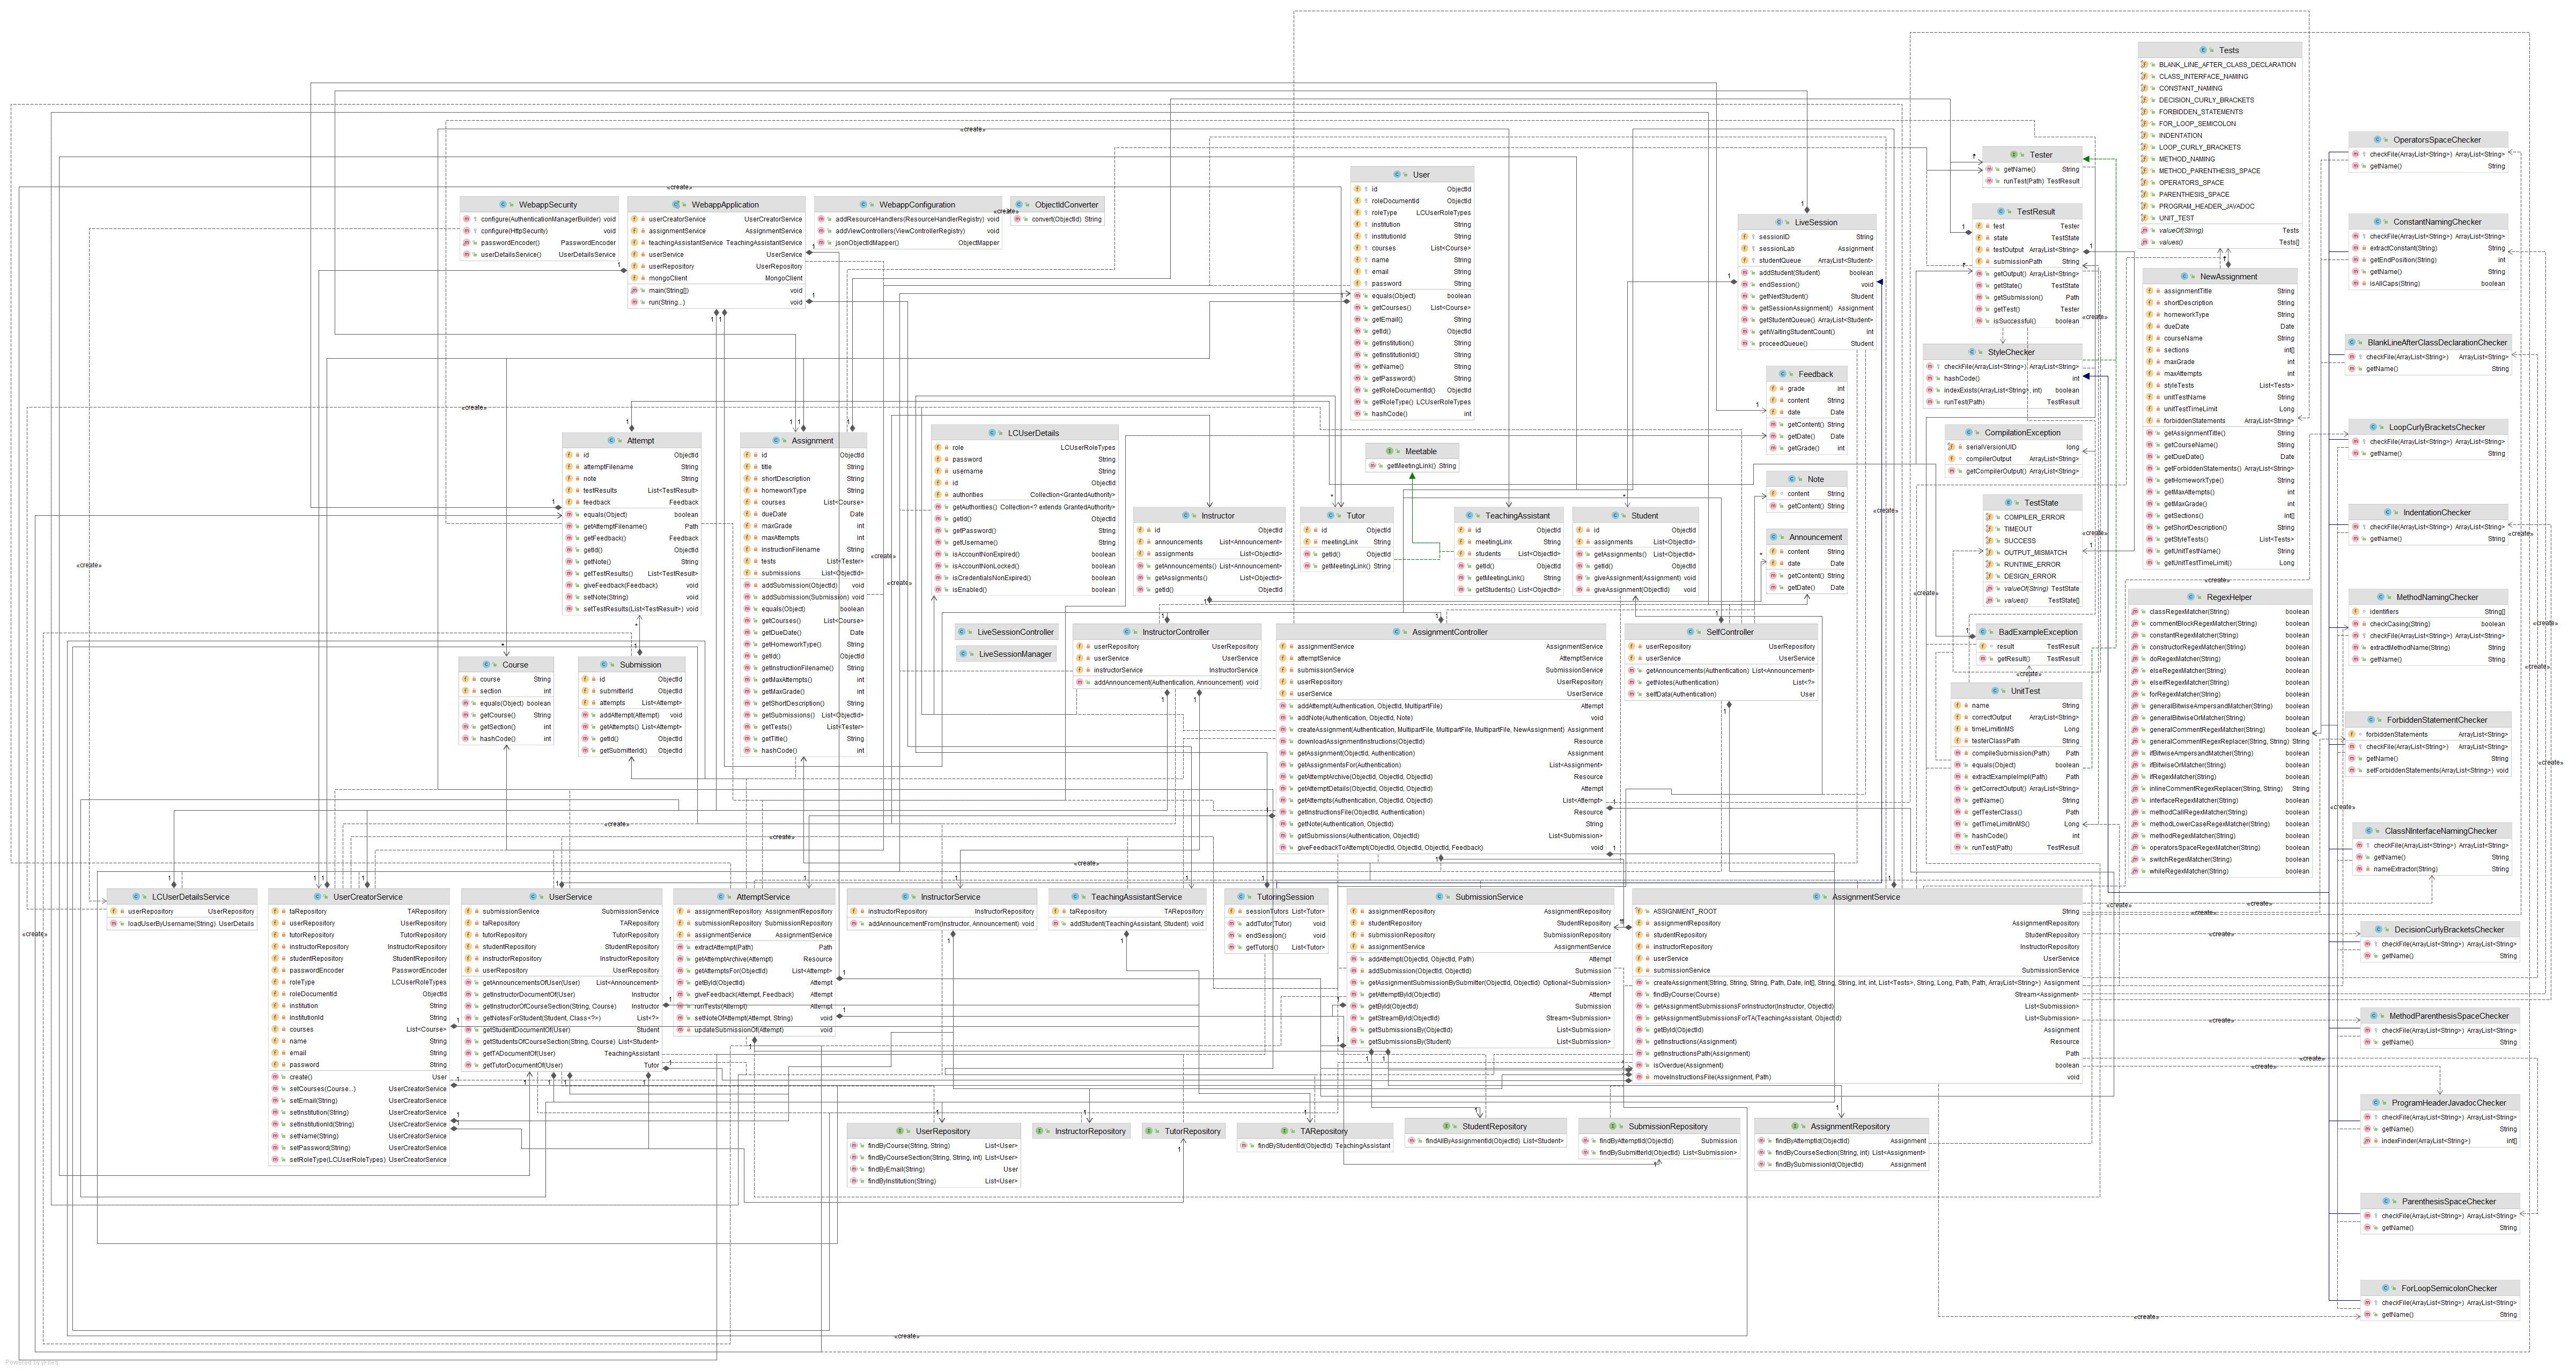
\includegraphics[width=\textwidth]{UML.jpg}
        \caption{UML Class Diagram for LabConnect}~\label{fig:class-diagram}
    \end{figure}

    
    \section{Task Assignment}
    
    The division of work for the model classes is as follows;
    
    \begin{table}[htbp!]
        \renewcommand{\arraystretch}{1.4}
        \centering
        \small
        \begin{tabular}{|p{0.25\textwidth}|p{0.25\textwidth}|p{0.25\textwidth}|p{0.25\textwidth}|p{0.25\textwidth}|}
            {\bf Borga Haktan Bilen} & {\bf Vedat Eren Arıcan} & {\bf Berkan Şahin} & {\bf Berk Çakar} & {\bf Alp Ertan} \\ \hline
            AssignmentController & NewAssignment & NewAssignment & Note & LiveSession \\ \hline
            SelfController & Note & AssignmentController & AssignmentController & LoopCurlyBracketsChecker \\ \hline
            AttemptService & AssignmentController & InstructorController & SelfController & RegexHelper \\ \hline
            Assignment & InstructorController & SelfController & Announcement & CompilationException \\ \hline
            Feedback & SelfController & AssignmentService & Course & \\ \hline
            Meetable & AssignmentService & AttemptService & LineAfterClassChecker & \\ \hline
            LineAfterClassChecker & AttemptService & SubmissionService & ConstantNamingChecker & \\ \hline
            ClassNamingChecker & Announcement & Assignment & DecisionBracketsChecker & \\ \hline
            IllegalStatementChecker & Attempt & Attempt & IllegalStatementChecker & \\ \hline
            MethodNamingChecker & Course & Submission & ForLoopSemicolonChecker & \\ \hline
            OperatorsSpaceChecker & Feedback & LiveSession & IndentationChecker & \\ \hline
            ProgramHeaderChecker & IllegalStatementChecker & LiveSessionManager & LoopCurlyBracketsChecker & \\ \hline
            RegexHelper & MethodNamingChecker & TutoringSession & MethodNamingChecker & \\ \hline
            Tester & RegexHelper & RegexHelper & MethodSpaceChecker & \\ \hline
            UserService & TestResult & StyleChecker & OperatorsSpaceChecker & \\ \hline
            Student & UserService & BadExampleException & ParenthesisSpaceChecker & \\ \hline
            TeachingAssistant & Tutor & TestResult & RegexHelper & \\ \hline
            Tutor & User & TestState & StyleChecker & \\ \hline
            User & InstructorRepository & UnitTest & UserService & \\ \hline
            InstructorRepository & StudentRepository & Instructor & & \\ \hline
            StudentRepository & SubmissionRepository & Student & & \\ \hline
            SubmissionRepository & TARepository & TeachingAssistant & & \\ \hline
            TARepository & TutorRepository & User & & \\ \hline
            TutorRepository & UserRepository & AssignmentRepository & & \\ \hline
            UserRepository & ObjectIdConverter & WebappSecurity & & \\ \hline
            & ObjectIdConverter & WebappConfiguration & & \\ \hline
            & WebappApplication & WebappApplication & & \\ \hline
            & InstructorService & LCUserDetailsService & & \\ \hline
            & & TeachingAssistantService & & \\ \hline
            & & UserCreatorService & & \\ \hline
        \end{tabular}
    \end{table}
    
    The division above is only for the implemented Java classes.
    As for the remaining work, we have decided to not limit anyone to work on a particular technology
    involved in the project. This project is, above all, intended for us to learn new technologies
    and gain experience for both teamwork and medium/large scale development. In which case, it works
    against this goal to have clean-cut distinctions in task assignment. 
    Theoretically, having all group members to strive to experience a variety of technologies should also ensure an even
    partition of work. Lastly, note that the project proposed thus far is of scale large enough to accommodate 
    members working on a specific component without clashing.
    
\end{document}

